\documentclass[12pt]{article}
\usepackage[utf8]{inputenc}
\usepackage[T1,T2A]{fontenc}
\usepackage[english,russian]{babel}
\usepackage{graphicx} % Allows you to insert figures
\usepackage{subcaption}
\usepackage{amsmath} % Allows you to do equations
\usepackage{fancyhdr} % Formats the header
\usepackage{geometry} % Formats the paper size, orientation, and margins
\usepackage{dirtytalk} % typesetting different types of quotation
\usepackage{csquotes}
\usepackage{hyperref}
\usepackage{listings}
\usepackage{xcolor}
\usepackage{array}
\usepackage{caption}
\usepackage{float}     % in preamble, for [H] placement
\usepackage{booktabs}   % For nicer tables
\usepackage{tikz}       % For diagrams
\usepackage{pgfgantt}   % For Gantt charts
\usetikzlibrary{shapes,arrows,positioning,fit,backgrounds}

% Code styling
\lstset{
    basicstyle=\ttfamily\footnotesize,
    backgroundcolor=\color{lightgray!20},
    keywordstyle=\color{blue},
    commentstyle=\color{green!50!black},
    stringstyle=\color{red},
    numbers=left,
    numberstyle=\tiny\color{gray},
    stepnumber=1,
    numbersep=10pt,
    showspaces=false,
    showstringspaces=false,
    showtabs=false,
    frame=single,
    tabsize=2,
    breaklines=true,
    breakatwhitespace=false,
    escapeinside={\%*}{*)},
    extendedchars=false,
    keepspaces=true,
    morekeywords={void, TaskHandle_t, TickType_t, xTaskCreate, vTaskDelay, vTaskDelayUntil, xSemaphoreGive, xSemaphoreTake, xSemaphoreCreateMutex, xSemaphoreCreateBinary, xTaskGetTickCount}
}

\linespread{1.25} % About 1.5 spacing in Word
\setlength{\parindent}{0.8cm} % No paragraph indents
\setlength{\parskip}{0em} % Paragraphs separated by one line
\renewcommand{\headrulewidth}{0pt} % Removes line in header
\geometry{a4paper, portrait, margin=1in}
\setlength{\headheight}{14.49998pt}
\graphicspath{ {../lib/lab3.2/plant_uml/img/} }

\begin{document}
\begin{titlepage}
	\thispagestyle{empty}
	
	\begin{center}
		\textsc{\large Ministry of Education of Republic of Moldova}\\[0.5cm]
		\textsc{\large Technical University of Moldova}\\[0.5cm]
		\textsc{\large Faculty of Computers, Informatics and Microelectronics}\\[0.5cm]
		\textsc{\large Department of Physics}\\[1.2cm]
	\end{center}

	\vspace{25 mm}

	\begin{center}
		\textsc{\large Embedded Systems}\\[0.5cm]
		\textsc{\large Laboratory work \#3.2}\\[0.5cm]

		\newcommand{\HRule}{\rule{\linewidth}{0.5mm}}
		\vspace{10 mm}
		\HRule \\[0.4cm]
		{ \LARGE \bfseries Dual Sensor Monitoring System with FreeRTOS - Analog Sound and Digital Temperature Acquisition}\\[0.4cm]
		\HRule \\[1.5cm]
	\end{center}

	\vspace{10mm}

	\begin{minipage}[t]{0.4\textwidth}
		\begin{flushleft} \large
			\emph{Author:} \\
			Dmitrii \textsc{Belih}\\
			std. gr. FAF-232
		\end{flushleft}
	\end{minipage}
	\hfill
	\begin{minipage}[t]{0.4\textwidth}
		\begin{flushright} \large
			\emph{Verified:} \\
			\textsc{Martiniuc} A.\\
		\end{flushright}
	\end{minipage}\\[3cm]

	\vspace{5 mm}
	\begin{center}
		\large Chișinău 2026\\[0.5cm]
	\end{center}

	\vfill
\end{titlepage}

\setcounter{page}{1}
\pagestyle{fancy}
\fancyhf{}
\rhead{\thepage}
\lhead{FAF-232 Belih Dmitrii; Laboratory Work 3.2}

% ============================================================================
% CHAPTER 1: INTRODUCTION
% ============================================================================
\section*{1. Introduction}

\subsection*{1.1. Purpose of the Laboratory Work}

The purpose of this laboratory work is to develop a real-time embedded system using FreeRTOS for monitoring two different sensor types: an analog sound sensor and a digital temperature sensor. The system demonstrates simultaneous acquisition from multiple sensors with different communication protocols, signal conditioning with filtering (median filter), and intelligent display management that automatically switches between sensor readings. Key objectives include implementing non-blocking sensor acquisition, applying signal filtering techniques, managing shared display resources between multiple data sources, achieving configurable acquisition periods (20-100 ms) with minimal latency, and providing visual feedback through RGB LED color coding for different system states.

\subsection*{1.2. Laboratory Objectives}

The specific objectives of this laboratory work include implementing periodic signal acquisition from an analog sound sensor and digital DS18B20 temperature sensor at configurable intervals (20-100 ms), developing signal conditioning with saturation, salt-and-pepper filtering, and median filter for noise reduction, implementing intelligent display management that shows temperature by default and switches to sound level when events are detected, utilizing FreeRTOS tasks with different priorities for sensor acquisition, signal processing, temperature reading, display updates, and RGB LED control, achieving input signal latency under 100 ms through precise task scheduling, implementing thread-safe access to shared display using mutexes for resource protection, and designing modular software architecture with clear separation between hardware abstraction and application logic.

% ============================================================================
% CHAPTER 2: ANALYSIS OF DOMAIN SITUATION
% ============================================================================
\section*{2. Analysis of Domain Situation and Technological Context}

\subsection*{2.1. Analog vs Digital Sensors}

Analog sensors provide continuous voltage signals that must be converted to digital values using an Analog-to-Digital Converter (ADC). The sound sensor used in this laboratory work outputs an analog voltage proportional to sound intensity, which is read by the ESP32's 12-bit ADC providing values from 0 to 4095. Digital sensors communicate via serial protocols such as I2C, SPI, UART, or proprietary interfaces. The DS18B20 temperature sensor uses the OneWire protocol, which allows communication over a single data line with ground and power connections. Digital sensors typically provide better noise immunity and higher accuracy but require more complex communication protocols.

\subsection*{2.2. Signal Filtering Techniques}

Noise in sensor readings can be addressed through various filtering techniques. Median filtering is particularly effective for removing salt-and-pepper noise (random outliers) while preserving edge information. In this implementation, a median filter with a window size of 5 samples is applied to temperature readings, which significantly reduces measurement noise without introducing phase delay characteristic of averaging filters. Weighted averaging can also be applied for smoothing signals, where recent samples have higher weights than older samples.

\subsection*{2.3. Non-Blocking I/O Operations}

Real-time systems must avoid blocking operations that prevent other tasks from executing. The DS18B20 temperature sensor requires approximately 750ms for temperature conversion at 12-bit resolution. To prevent blocking the entire system, the temperature acquisition is split into two phases: requesting conversion and reading the result. This allows other tasks to continue executing during the conversion period, maintaining system responsiveness.

\subsection*{2.4. Display Resource Management}

When multiple data sources compete for the same display resource, intelligent management is required. This system implements a priority-based display scheme where temperature is shown by default (every 500ms), but when sound events are detected, the display immediately switches to show the sound level for 2 seconds before returning to temperature monitoring. This ensures both regular monitoring and immediate feedback for time-critical events.

\subsection*{2.5. RGB LED Color Coding}

RGB LEDs provide multi-state visual feedback beyond simple on/off indication. In this system, the RGB LED indicates different system states: red for idle/normal operation, green for sound detection events, and can be extended with other colors for different alert levels. PWM control allows smooth color transitions and intensity variations for more sophisticated status indication.

% ============================================================================
% CHAPTER 3: RESOURCES AND MATERIALS
% ============================================================================
\section*{3. Resources and Materials}

\subsection*{3.1. Hardware Resources}

\begin{table}[H]
	\centering
	\caption{Hardware Components}
	\label{tab:hardware-resources}
	\begin{tabular}{|l|l|l|}
		\hline
		\textbf{Component} & \textbf{Specification} & \textbf{Quantity} \\
		\hline
		ESP32 DevKit V1 & Dual-core 240MHz, 520KB SRAM, 4MB Flash & 1 \\
		\hline
		Sound Sensor Module & Analog A0 (GPIO 34), Digital D0 (GPIO 12) & 1 \\
		\hline
		Temperature Sensor & DS18B20, OneWire protocol, GPIO 4 & 1 \\
		\hline
		RGB LED & Red/Green/Blue pins: GPIO 25/26/27 & 1 \\
		\hline
		LCD 16×2 & I2C interface, Address 0x27 & 1 \\
		\hline
		Pull-up Resistor & 4.7k$\Omega$ for OneWire bus & 1 \\
		\hline
		Breadboard & 400/830 tie-points & 1 \\
		\hline
		Jumper Wires & Male-to-male, Male-to-female & ~25 \\
		\hline
		USB Cable & Micro-USB for power/programming & 1 \\
		\hline
	\end{tabular}
\end{table}

\subsection*{3.2. Software Resources}

\begin{table}[H]
	\centering
	\caption{Software Tools and Frameworks}
	\label{tab:software-resources}
	\begin{tabular}{|l|l|l|}
		\hline
		\textbf{Tool/Framework} & \textbf{Version/Platform} & \textbf{Purpose} \\
		\hline
		PlatformIO & Latest & Build system, library management \\
		\hline
		FreeRTOS & 10.4.6 & Real-time operating system kernel \\
		\hline
		Arduino Framework & ESP32 & Hardware abstraction, GPIO, I2C, ADC \\
		\hline
		OneWire Library & 2.3.8 & DS18B20 temperature sensor communication \\
		\hline
		VS Code & Latest & Code editor with PlatformIO extension \\
		\hline
		Git & 2.43.0 & Version control \\
		\hline
		Serial Monitor & Built-in & Debugging output display \\
		\hline
	\end{tabular}
\end{table}

% ============================================================================
% CHAPTER 4: LABORATORY TASK DESCRIPTION
% ============================================================================
\section*{4. Laboratory Task Description}

\subsection*{4.1. Problem Statement}

Develop a real-time embedded system using FreeRTOS for monitoring two sensors: an analog sound sensor and a digital DS18B20 temperature sensor. The system must periodically acquire raw data from both sensors at configurable rates (20-100 ms), implement signal conditioning with saturation, salt-and-pepper filtering, and median filter for noise reduction, display processed values on LCD with intelligent switching between temperature and sound readings, provide visual feedback through RGB LED color coding for different system states, achieve real-time responsiveness with input latency under 100 ms, use FreeRTOS for task management with appropriate priorities, implement thread-safe access to shared LCD using mutexes, and demonstrate proper inter-task communication through semaphores for event signaling.

\subsection*{4.2. Functional Requirements}

\begin{table}[H]
	\centering
	\caption{Functional Requirements}
	\label{tab:functional-requirements}
	\begin{tabular}{|l|l|}
		\hline
		\textbf{Requirement} & \textbf{Description} \\
		\hline
		Sound Acquisition & Periodically read analog values from sound sensor (20-100 ms) \\
		\hline
		Temperature Acquisition & Non-blocking DS18B20 temperature reading (100ms cycle) \\
		\hline
		Signal Conditioning & Apply median filter (5 samples) to temperature readings \\
		\hline
		Display Management & Show temperature by default, switch to sound on events \\
		\hline
		Sound Detection & Detect when sound exceeds configurable threshold (1500) \\
		\hline
		RGB LED Feedback & Red for idle, Green for sound detection \\
		\hline
		Thread Safety & Mutex protection for shared LCD resource \\
		\hline
	\end{tabular}
\end{table}

\subsection*{4.3. Non-Functional Requirements}

\begin{table}[H]
	\centering
	\caption{Non-Functional Requirements}
	\label{tab:non-functional-requirements}
	\begin{tabular}{|l|l|l|}
		\hline
		\textbf{Requirement} & \textbf{Target} & \textbf{Acceptance Criteria} \\
		\hline
		Input Latency & $<$ 100ms & Oscilloscope measurement \\
		\hline
		Acquisition Period & 20-100 ms (configurable) & FreeRTOS task timing \\
		\hline
		Temperature Conversion & $<$ 800ms (non-blocking) & DS18B20 specification \\
		\hline
		Display Update Rate & 100 ms (sound), 500 ms (temp) & FreeRTOS task timing \\
		\hline
		Task Scheduling & Preemptive priority-based & FreeRTOS scheduler \\
		\hline
		Thread Safety & Mutex protection & No LCD corruption \\
		\hline
		Filter Response & 5-sample median & Stable temperature readings \\
		\hline
		Resource Efficiency & Minimal overhead & RAM $<$ 50KB \\
		\hline
	\end{tabular}
\end{table}

% ============================================================================
% CHAPTER 5: ARCHITECTURAL DESIGN
% ============================================================================
\section*{5. Architectural Design and Behavioral Modeling}

\subsection*{5.1. System Architecture}

The dual sensor monitoring system implements a layered architecture with four main components: Application Layer containing four FreeRTOS tasks for sound detection, temperature acquisition, display management, and RGB LED control, Synchronization Layer providing binary semaphores for inter-task communication and mutex for LCD resource protection, Kernel Primitives Layer offering wrapper classes for FreeRTOS API functions, and Hardware Abstraction Layer including device drivers for sound sensor, DS18B20 temperature sensor, RGB LED, and LCD display.

\subsection*{5.2. Component Diagram}

\begin{figure}[H]
    \centering
    
\includegraphics[width=0.9\textwidth]{02_component.png}
    \caption{FreeRTOS Application Component Diagram - Dual Sensor System}    \label{fig:component-diagram}
\end{figure}

This diagram shows the hierarchical structure of the system with application tasks, synchronization primitives, kernel wrappers, and hardware abstraction layers.

\subsection*{5.3. Task Activity Diagrams}

\subsubsection*{vTaskDetect Activity Diagram}

\begin{figure}[H]
    \centering
    
\includegraphics[width=0.3\textwidth]{04_activity_detect.png}
    \caption{Activity Diagram - Sound Detection Task}
    \label{fig:activity-detect}
\end{figure}

The diagram illustrates the 20ms periodic cycle of sound sensor reading, threshold comparison, and event signaling. It shows how the task continuously monitors the sound sensor and triggers appropriate responses when the threshold is exceeded.

The vTaskDetect task runs every 20ms at priority 3, reading analog sound values from GPIO 34, implementing rising edge detection with configurable threshold of 1500, applying 2000ms interval between detections to prevent spamming, updating shared data with current sound level, and triggering RGB LED change to green when sound events occur.

\subsubsection*{vTaskTemperature Activity Diagram}

\begin{figure}[H]
    \centering
    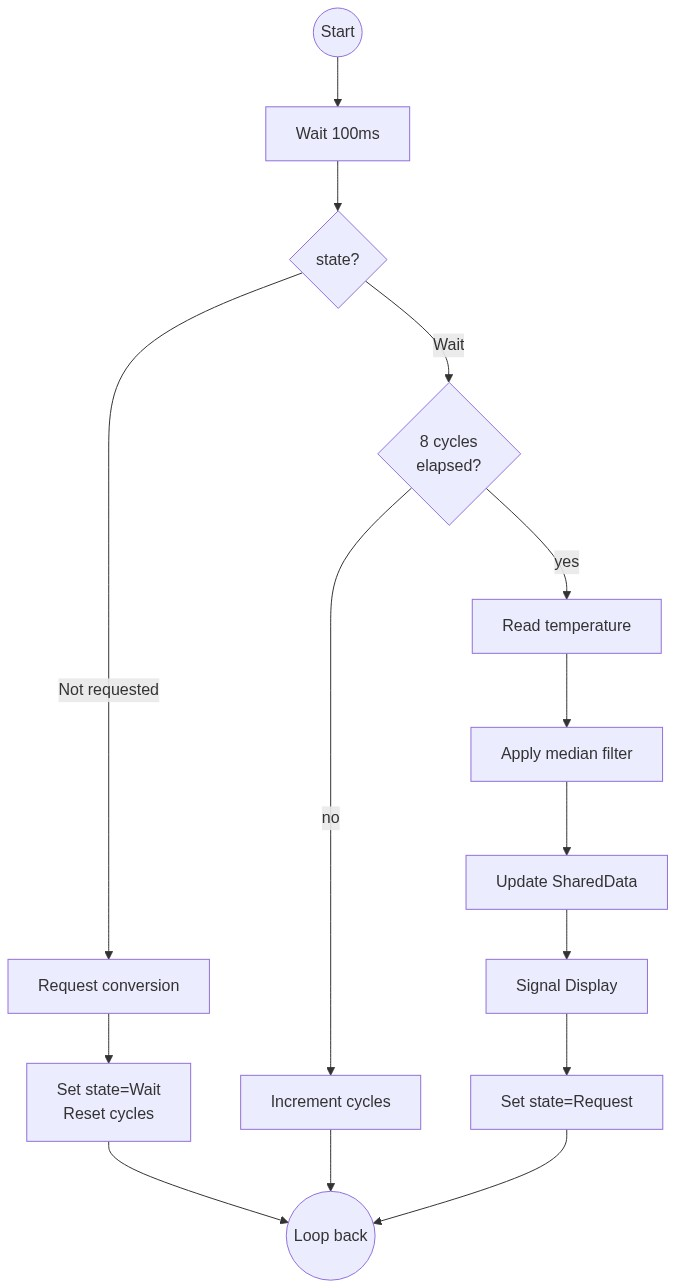
\includegraphics[width=0.3\textwidth]{05_activity_temperature.png}
    \caption{Activity Diagram - Temperature Acquisition Task}
    \label{fig:activity-temperature}
\end{figure}

This flowchart shows the non-blocking temperature reading process with OneWire communication and median filtering. The task requests temperature conversion and reads the result after 8 cycles without blocking other system operations.

The vTaskTemperature task runs every 100ms at priority 3, requesting temperature conversion from DS18B20 via OneWire protocol, waiting for 8 cycles (800ms) for conversion to complete without blocking, reading temperature value, applying 5-sample median filter for noise reduction, storing both raw and filtered values in shared data, and updating display semaphore to signal new reading available.

\subsubsection*{vTaskDisplay Activity Diagram}

\begin{figure}[H]
    \centering
    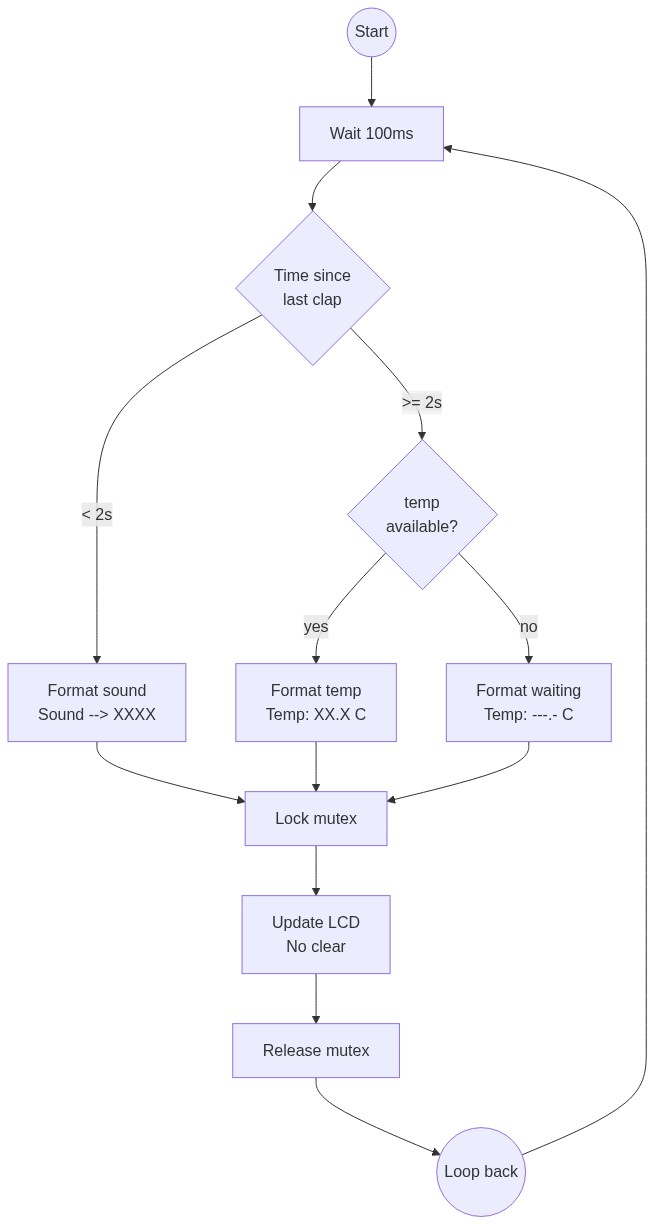
\includegraphics[width=0.3\textwidth]{06_activity_display.png}
    \caption{Activity Diagram - Display Management Task}
    \label{fig:activity-display}
\end{figure}

The diagram demonstrates intelligent display switching between temperature monitoring and sound event visualization. The task checks for recent sound events and updates the LCD accordingly to show the most relevant information.

The vTaskDisplay task runs every 100ms at priority 2, checking for sound event timestamp to determine display mode, showing sound level "Sound --> XXXX" when recent event detected (within 2000ms), showing temperature "Temp: XX.X C" / "Filt: XX.X C" when no recent events, acquiring mutex for LCD I2C access, and updating display with appropriate information without clearing entire screen.

\subsubsection*{vTaskRGBLED Activity Diagram}

\begin{figure}[H]
    \centering
    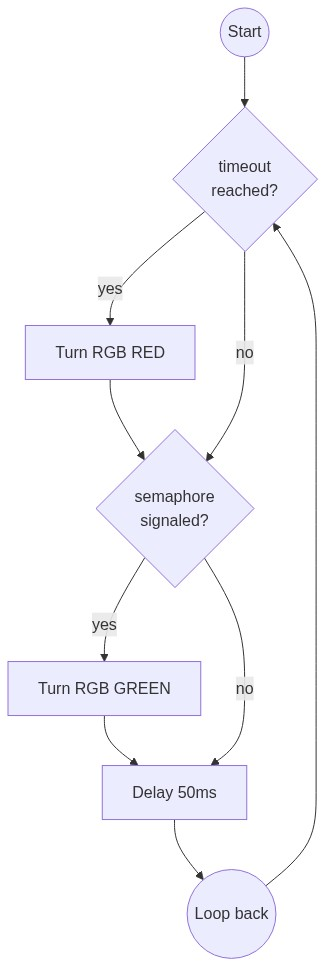
\includegraphics[width=0.3\textwidth]{07_activity_led.png}
    \caption{Activity Diagram - RGB LED Control Task}
    \label{fig:activity-led}
\end{figure}

This diagram illustrates the RGB LED state machine with red idle mode and green detection mode with timeout. The task continuously monitors for sound events and changes the LED color accordingly.

The vTaskRGBLED task runs continuously at priority 1, checking for sound event semaphore signals, setting RGB LED to green for 1000ms when sound detected, returning RGB LED to red color after timeout, implementing PWM control for smooth color transitions, and providing continuous visual feedback for system status.

\subsection*{5.4. Data Flow Architecture}

\begin{figure}[H]
    \centering
    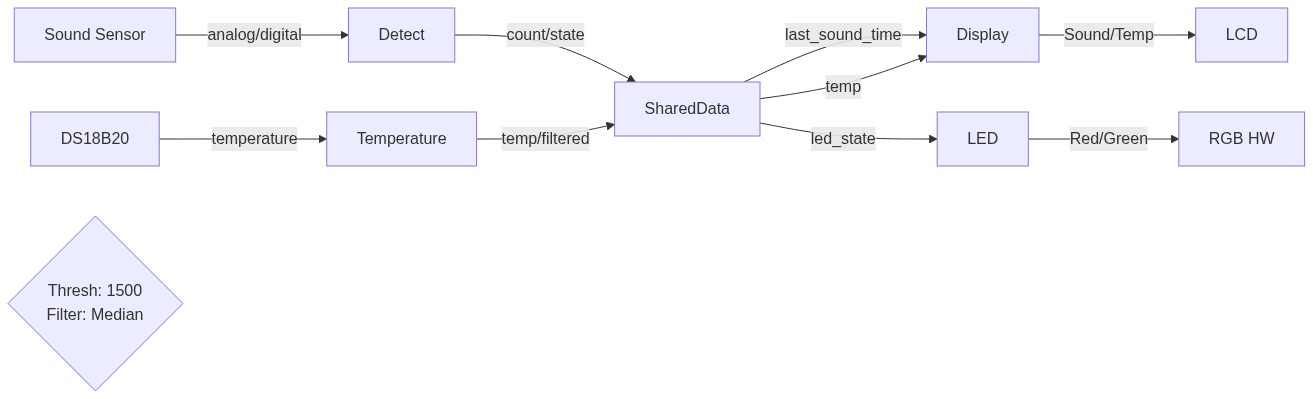
\includegraphics[width=0.9\textwidth]{08_dataflow.png}
    \caption{Data Flow - System Overview}
    \label{fig:dataflow-overview}
\end{figure}

This diagram shows the overall data flow from sensors through processing to output devices. It illustrates how data moves through different layers of the system architecture.

\begin{figure}[H]
    \centering
    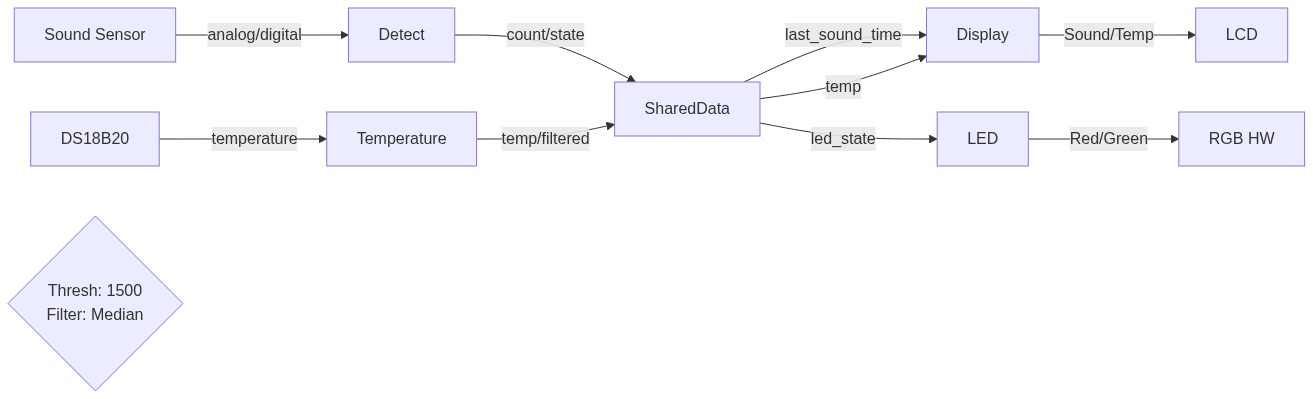
\includegraphics[width=0.7\textwidth]{08_dataflow.png}
    \caption{Data Flow - Sound and Temperature Sensors}
    \label{fig:dataflow-sensors}
\end{figure}

This diagram illustrates the input layer with analog sound sensor and digital temperature sensor acquisition. Both sensors provide data to the processing layer for further analysis.

\begin{figure}[H]
    \centering
    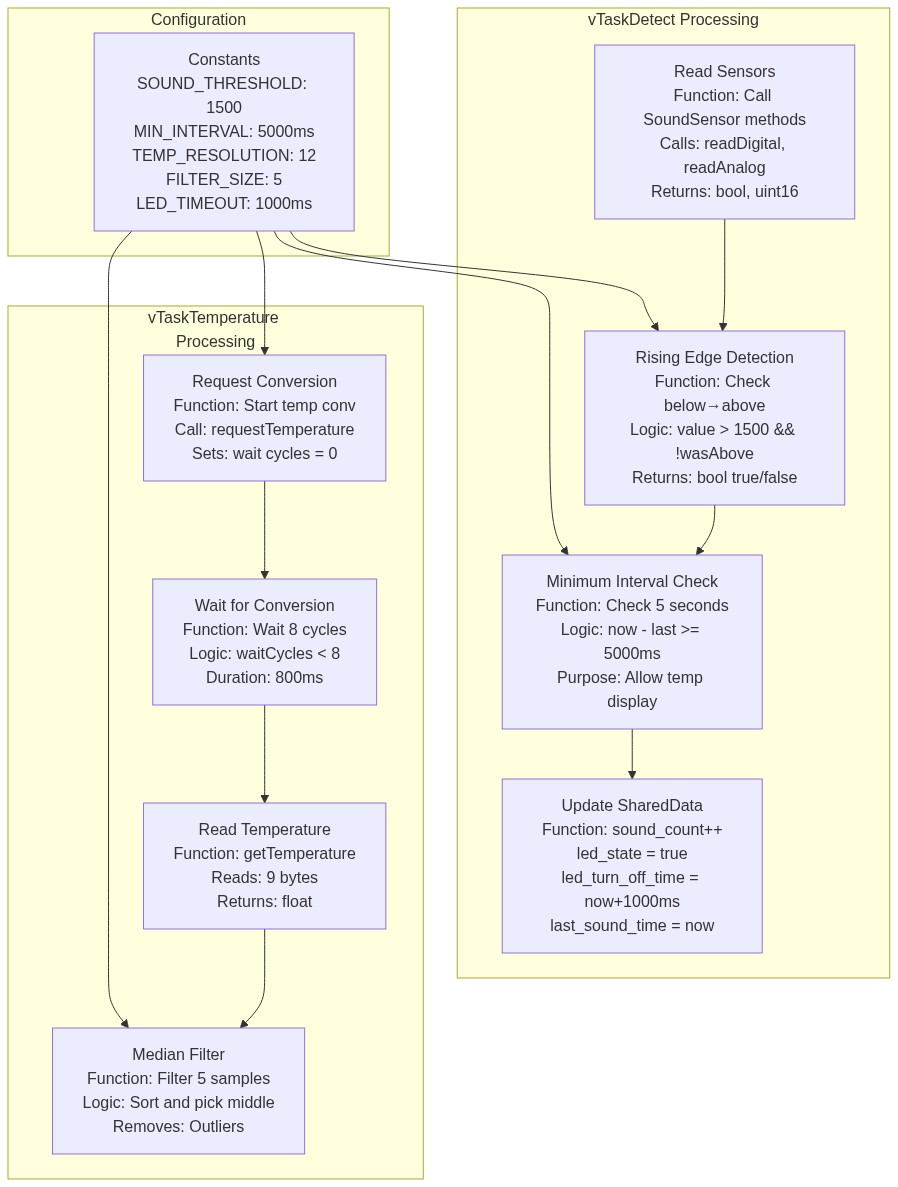
\includegraphics[width=0.7\textwidth]{17_dataflow_processing.png}
    \caption{Data Flow - Signal Processing Layer}
    \label{fig:dataflow-processing}
\end{figure}

The diagram shows signal conditioning with median filtering and threshold detection algorithms. Raw sensor data is processed to remove noise and detect events.



\begin{figure}[H]
    \centering
    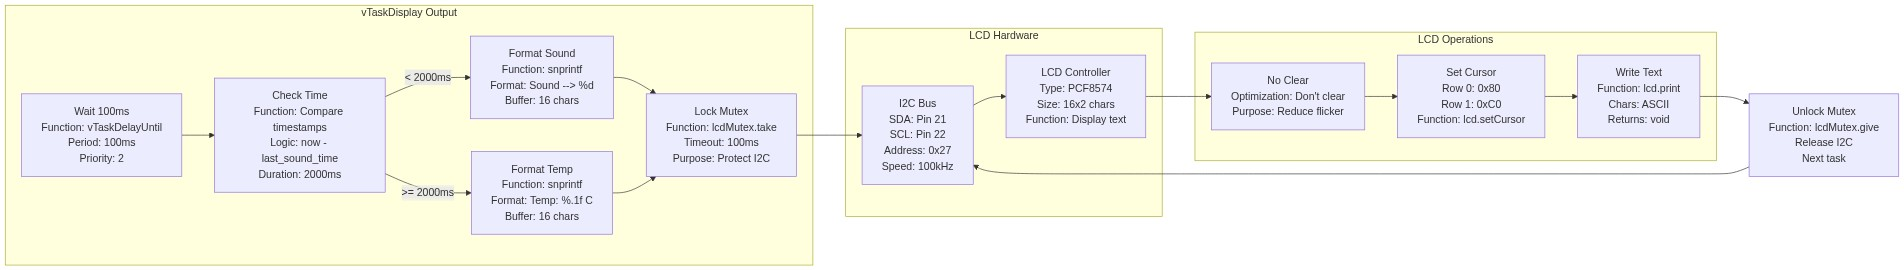
\includegraphics[width=0.7\textwidth]{19_dataflow_display.png}
    \caption{Data Flow - Display Output}
    \label{fig:dataflow-display}
\end{figure}

This diagram illustrates the LCD display update mechanism with mutex protection and mode switching. The display task safely accesses the shared data structure to show system information.

\begin{figure}[H]
    \centering
    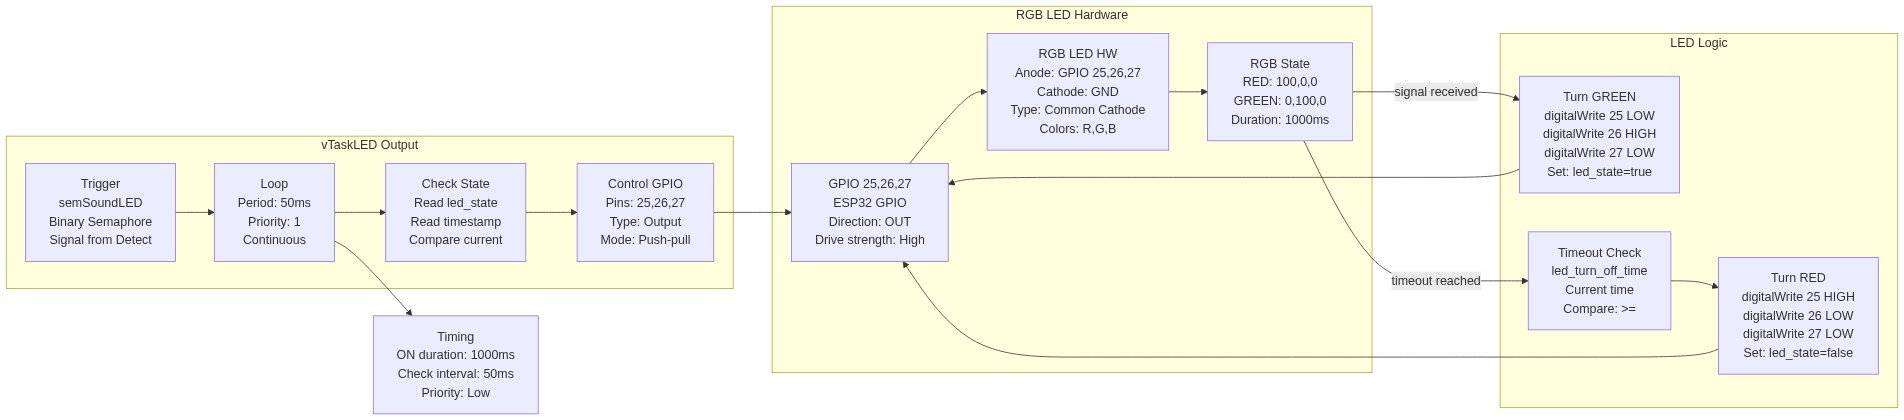
\includegraphics[width=0.7\textwidth]{20_dataflow_rgb_led.png}
    \caption{Data Flow - RGB LED Output}
    \label{fig:dataflow-led}
\end{figure}

The diagram shows RGB LED control logic with color transitions and timeout-based state changes. The LED task provides visual feedback for system status and events.

\subsection*{5.5. Sequence Diagrams}

\begin{figure}[H]
    \centering
    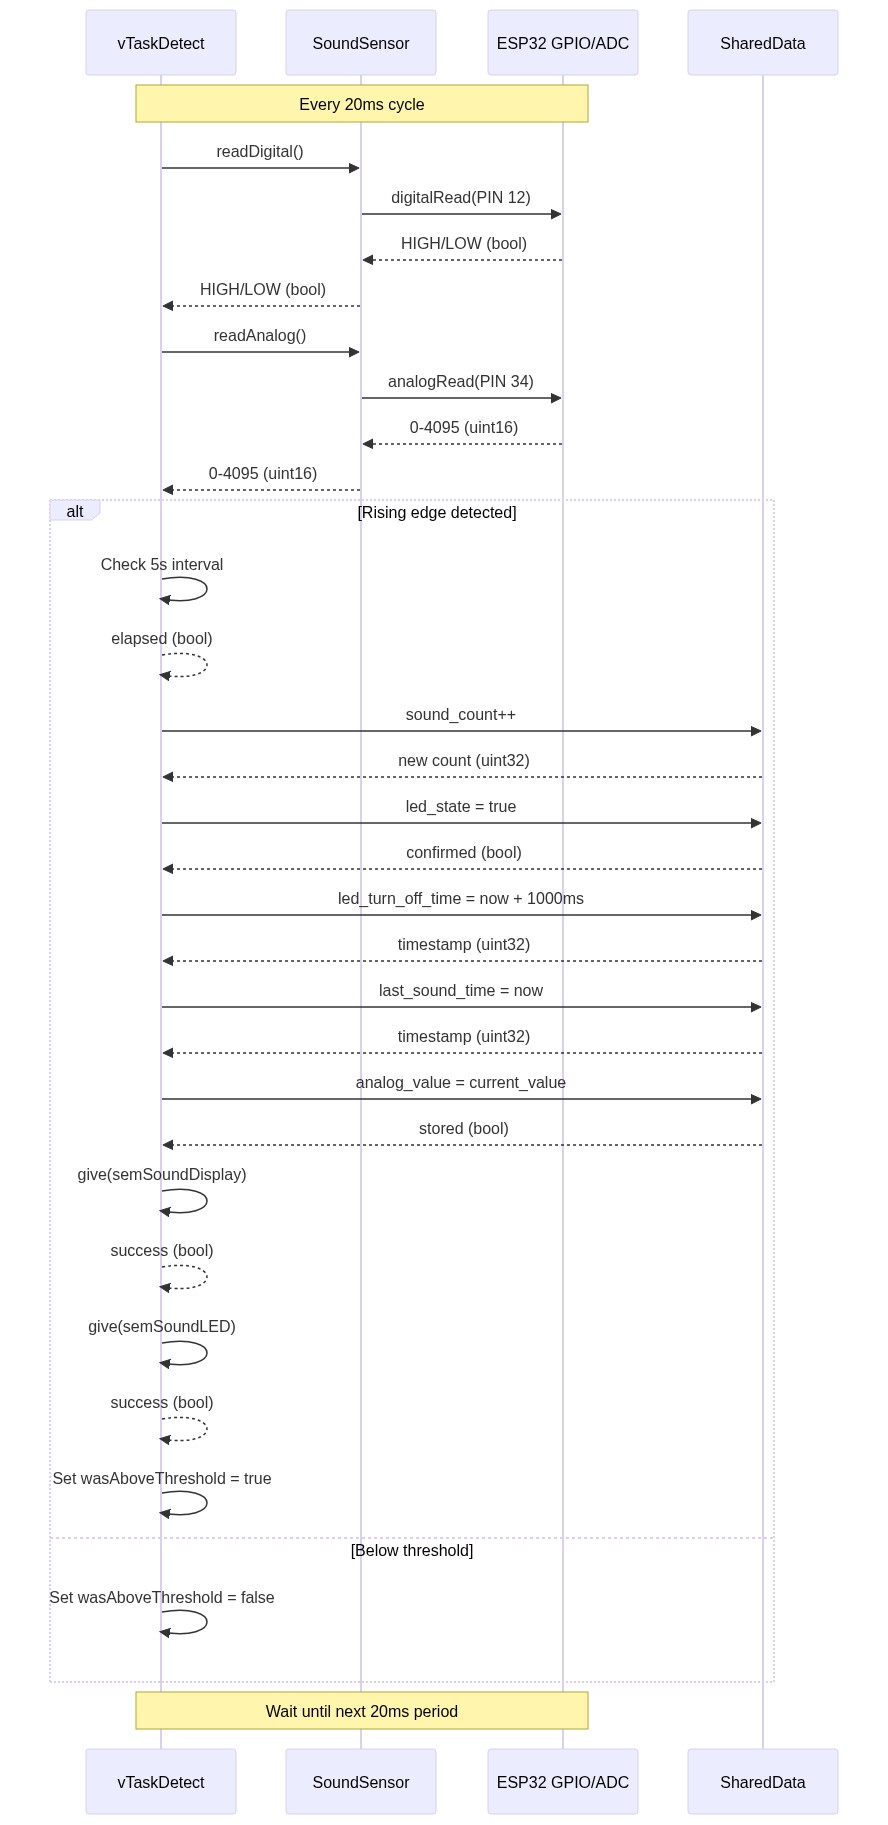
\includegraphics[width=0.8\textwidth]{11_sequence_sound_sensor.png}
    \caption{Sequence Diagram - Sound Sensor Acquisition}
    \label{fig:sequence-sound}
\end{figure}

This sequence diagram shows the interaction between vTaskDetect, SoundSensor driver, and shared data structure. It illustrates how the task reads sensor values and updates the shared state.

\begin{figure}[H]
    \centering
    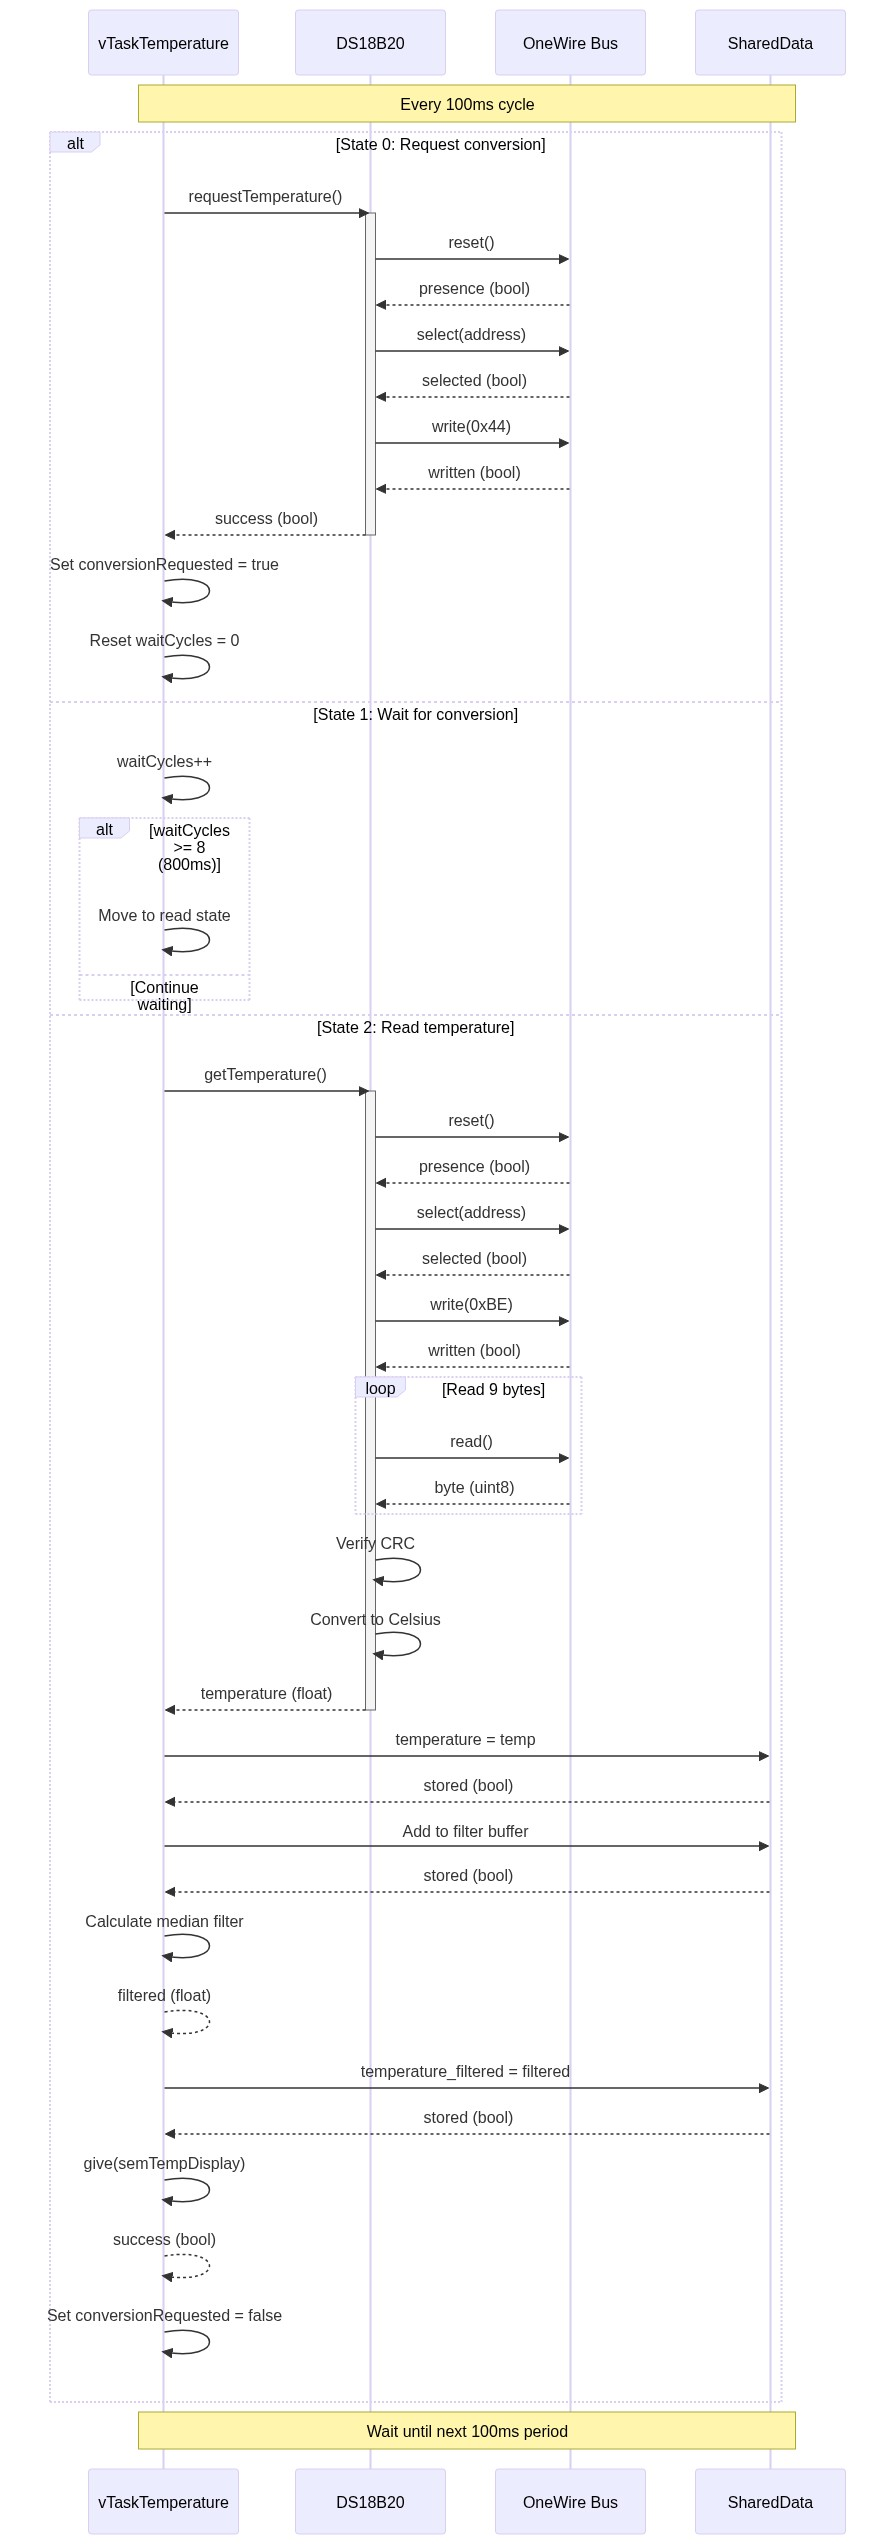
\includegraphics[width=0.8\textwidth]{12_sequence_temperature_sensor.png}
    \caption{Sequence Diagram - Temperature Sensor Acquisition}
    \label{fig:sequence-temperature}
\end{figure}

The diagram illustrates the non-blocking OneWire communication with DS18B20 temperature sensor. It shows the two-phase process of requesting conversion and reading the result.

\begin{figure}[H]
    \centering
    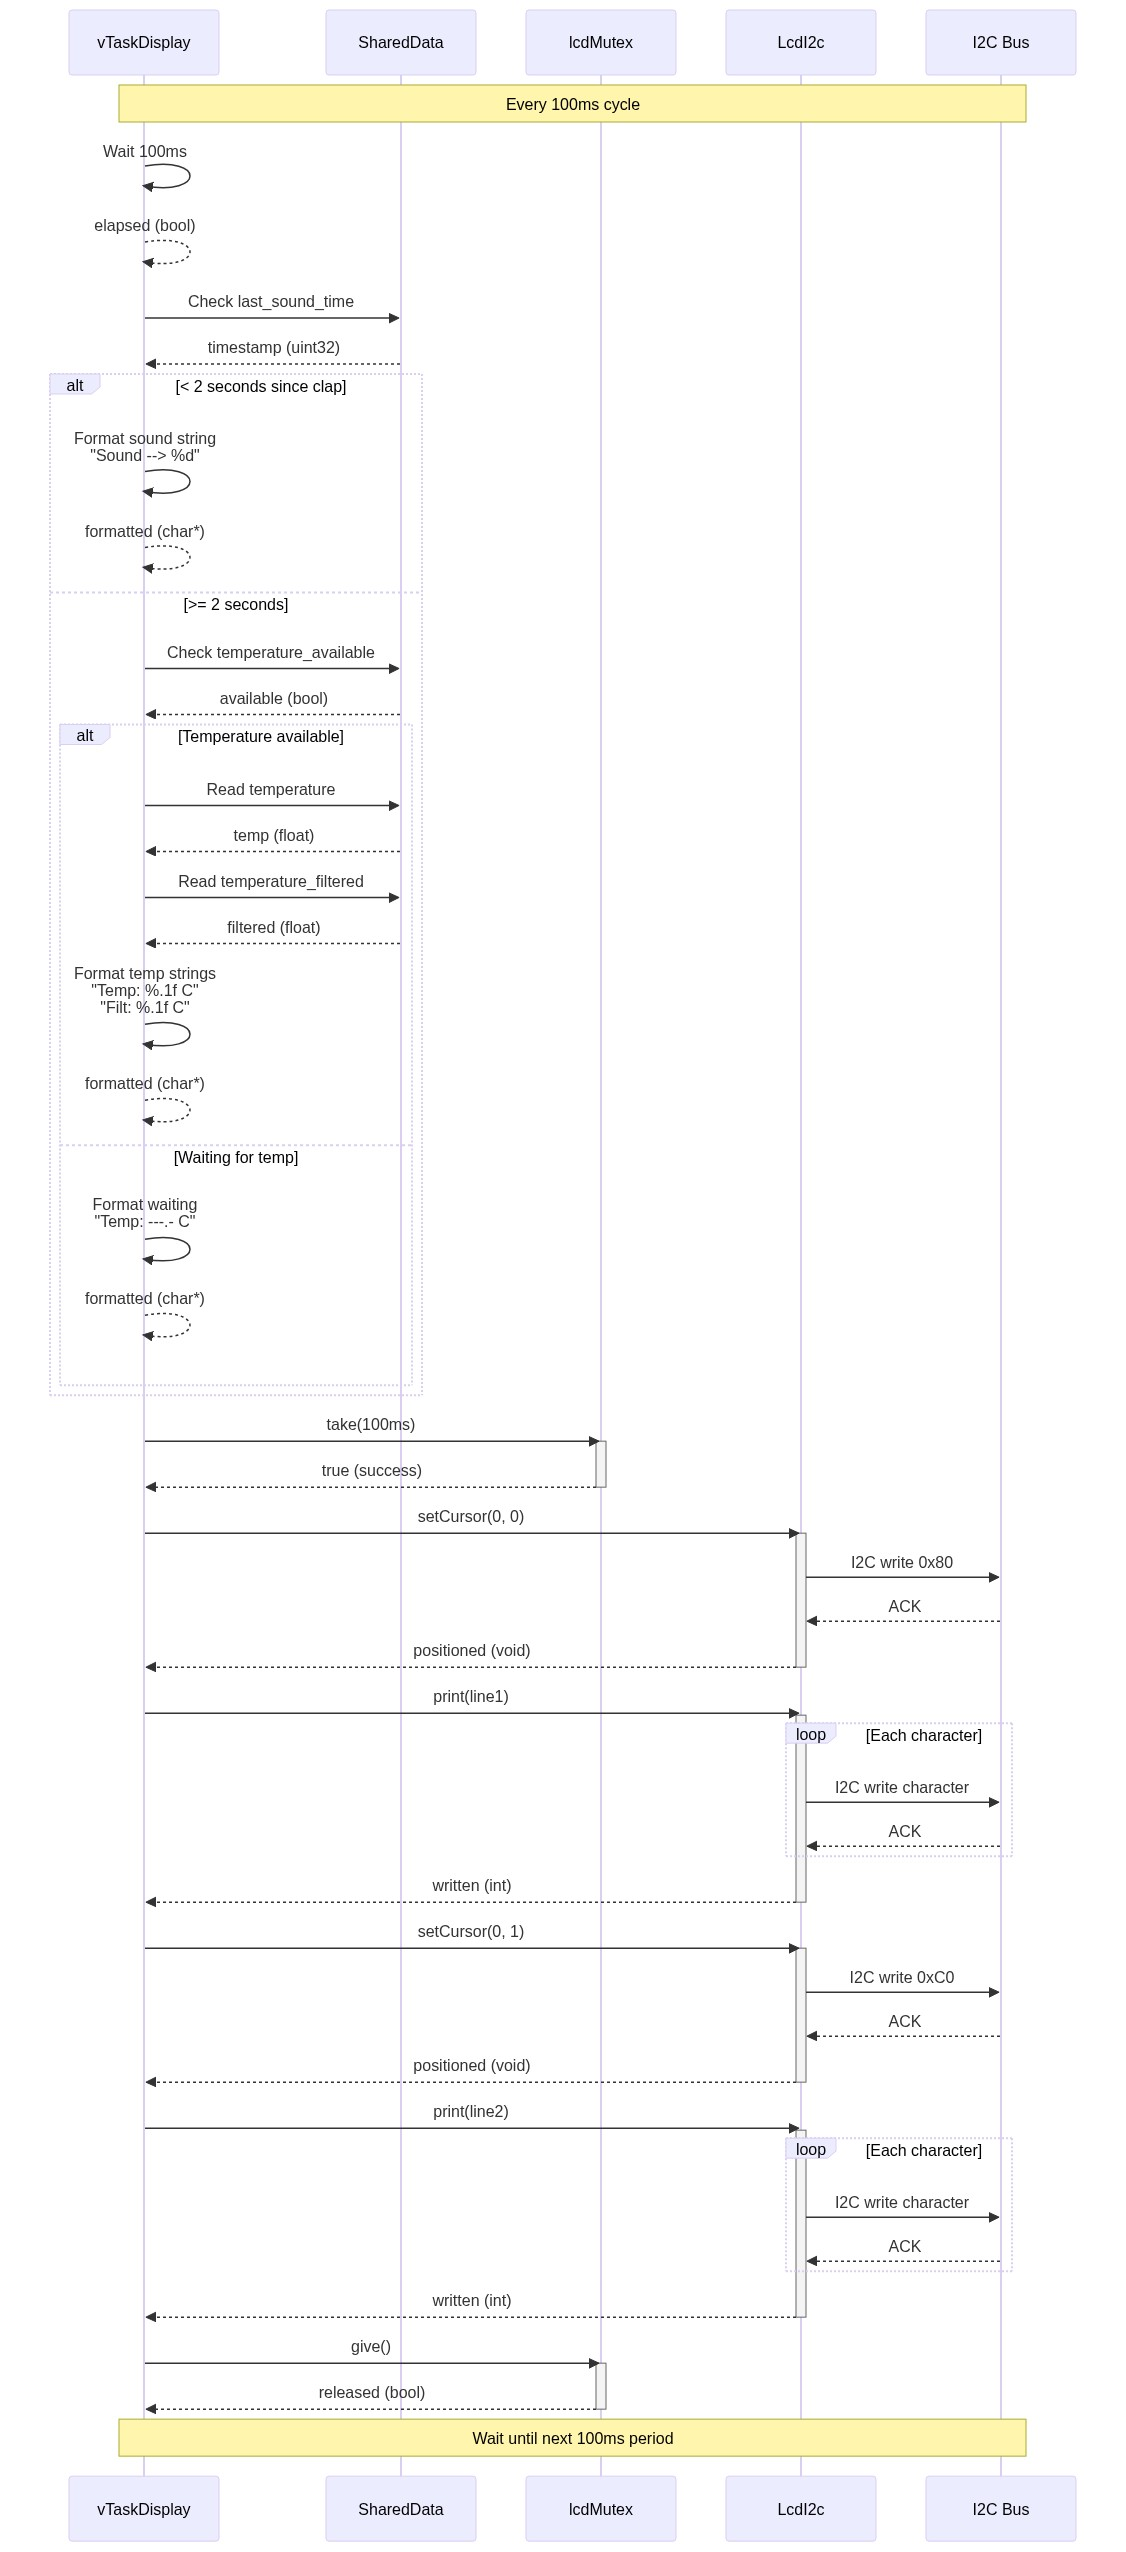
\includegraphics[width=0.8\textwidth]{13_sequence_lcd.png}
    \caption{Sequence Diagram - LCD Display Updates}
    \label{fig:sequence-lcd}
\end{figure}

This sequence diagram shows mutex-protected LCD I2C communication and display update process. It demonstrates how the display task safely updates the LCD without interference from other tasks.

\begin{figure}[H]
    \centering
    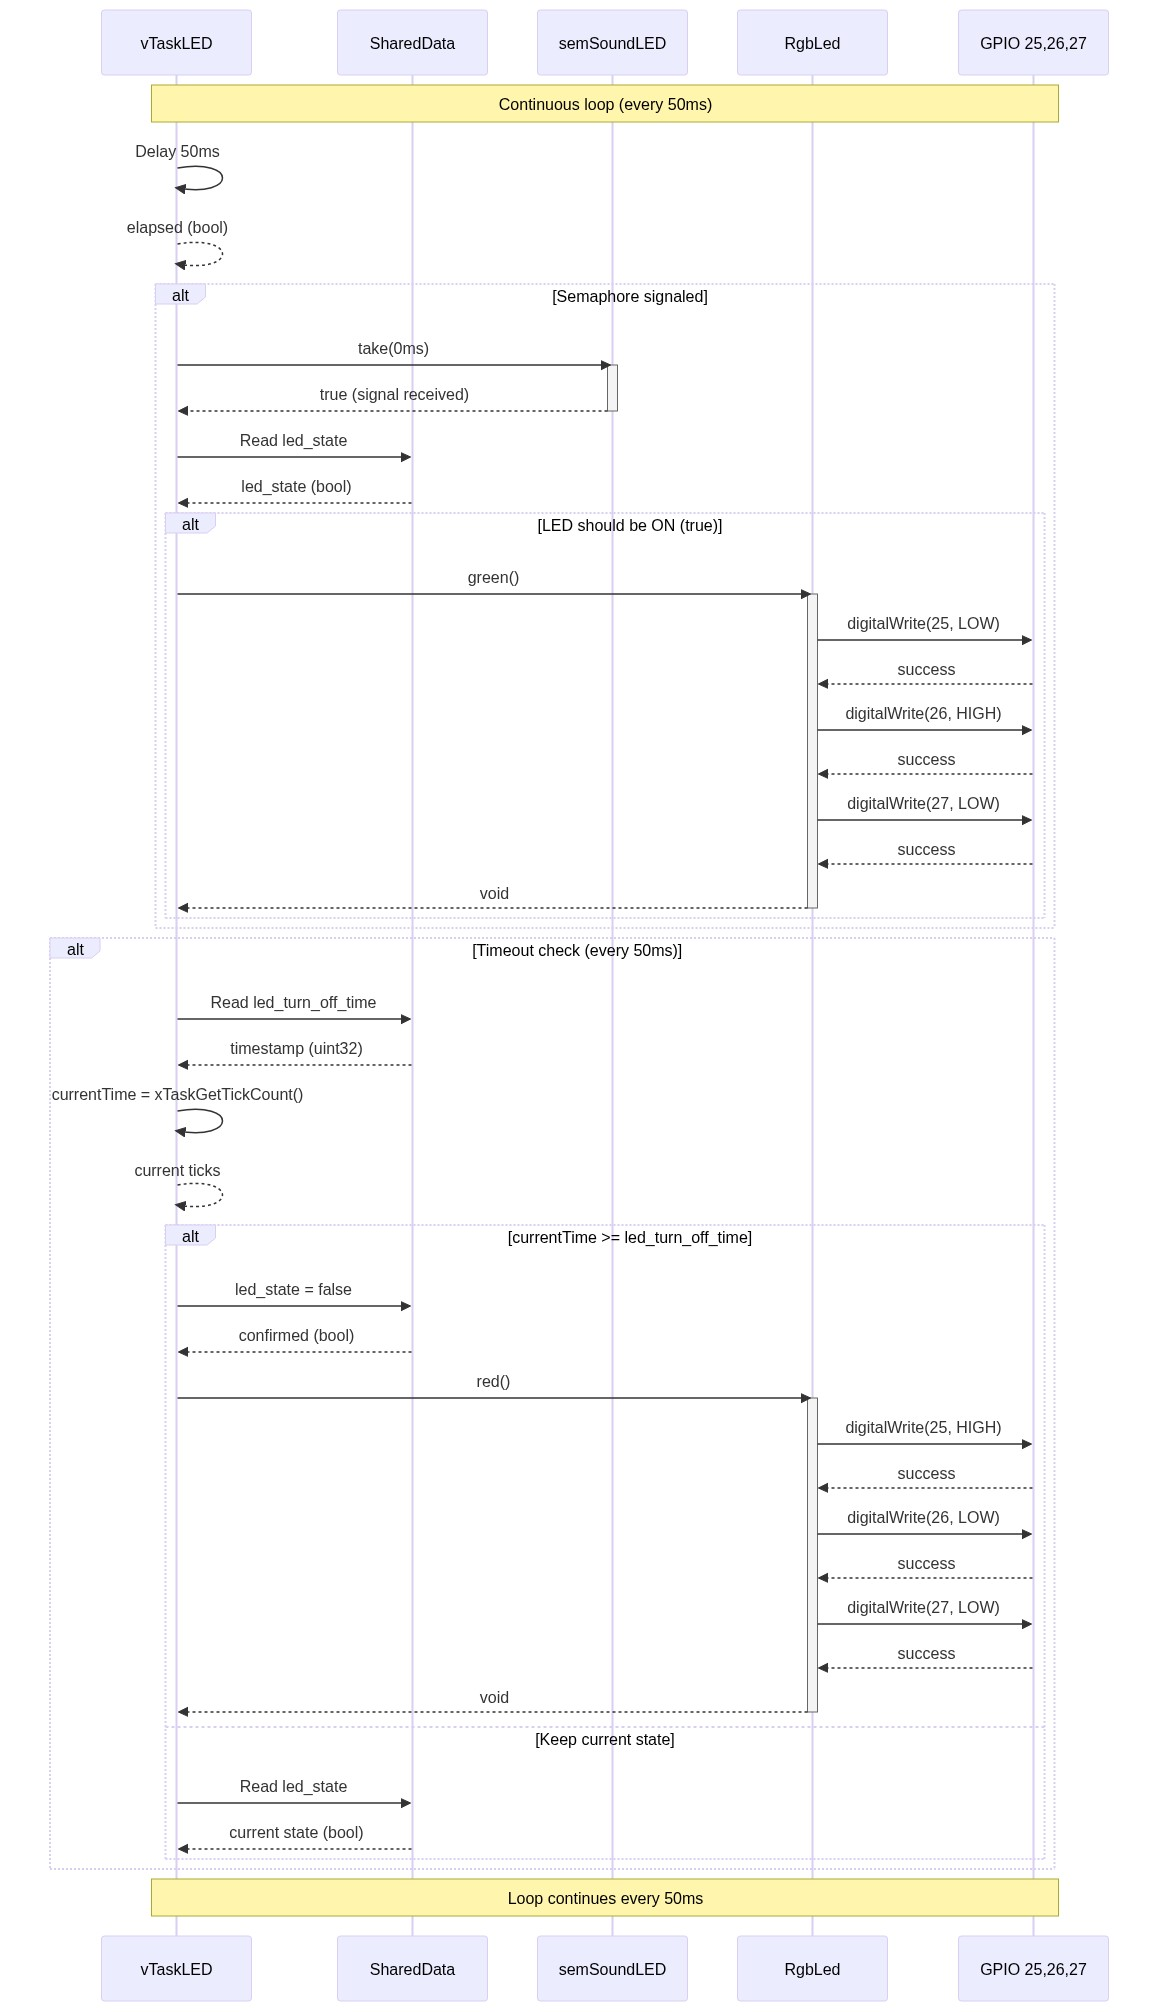
\includegraphics[width=0.8\textwidth]{14_sequence_rgb_led.png}
    \caption{Sequence Diagram - RGB LED Control}
    \label{fig:sequence-rgb}
\end{figure}

The diagram demonstrates RGB LED state transitions triggered by semaphore signals and timeout events. It shows how the LED task responds to sound detection events and returns to idle state.

\begin{figure}[H]
    \centering
    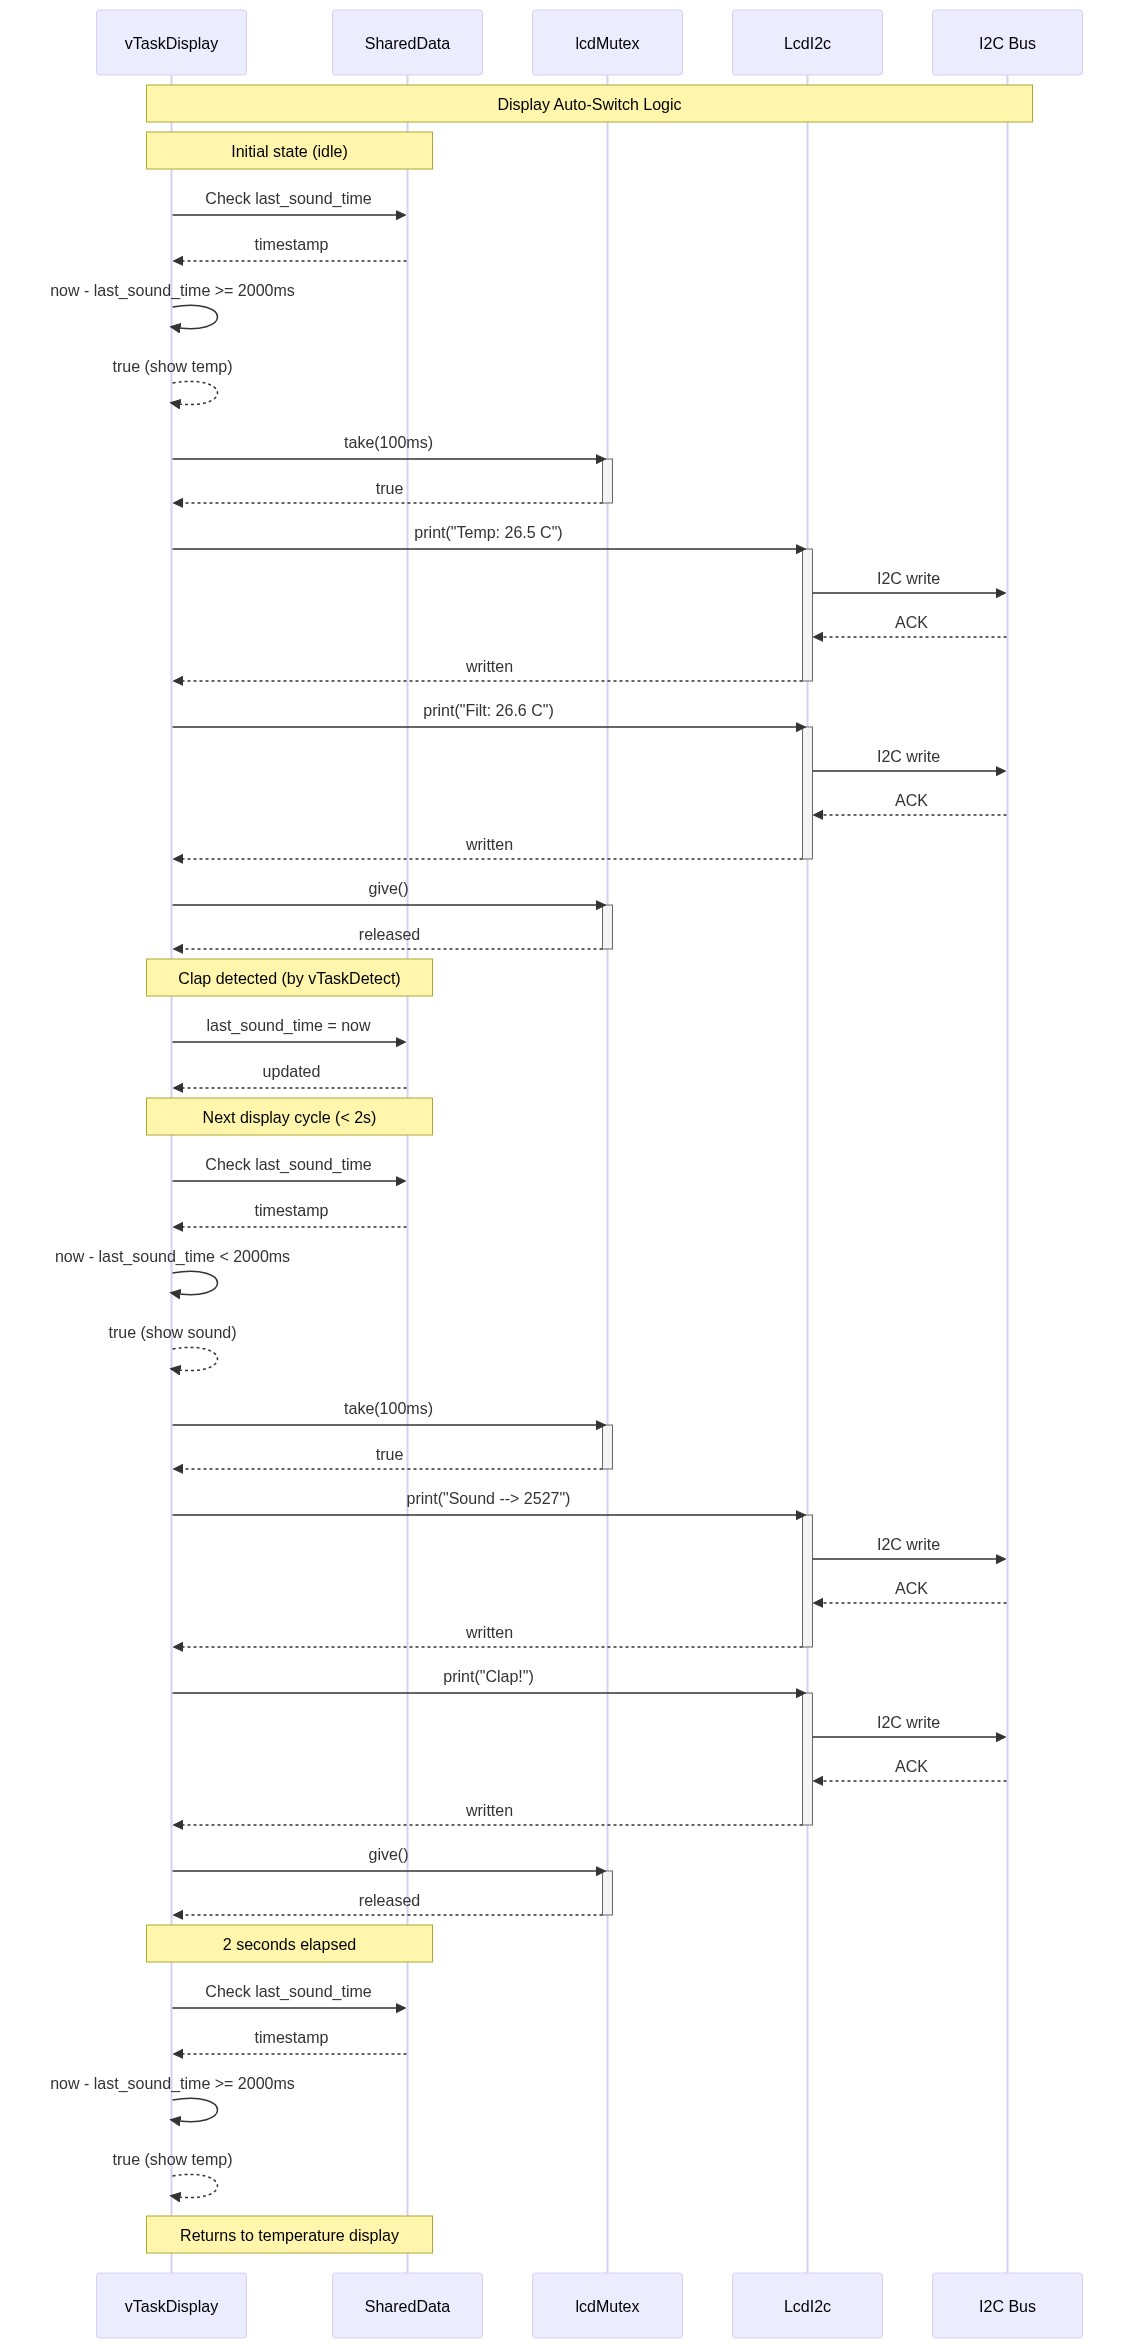
\includegraphics[width=0.8\textwidth]{22_sequence_display_switch.png}
    \caption{Sequence Diagram - Display Mode Switching}
    \label{fig:sequence-switch}
\end{figure}

This sequence diagram shows the automatic display switching between temperature and sound event modes. It illustrates how the system prioritizes time-critical sound events while maintaining regular temperature monitoring.

\subsection*{5.6. State Machine Diagrams}

\begin{figure}[H]
    \centering
    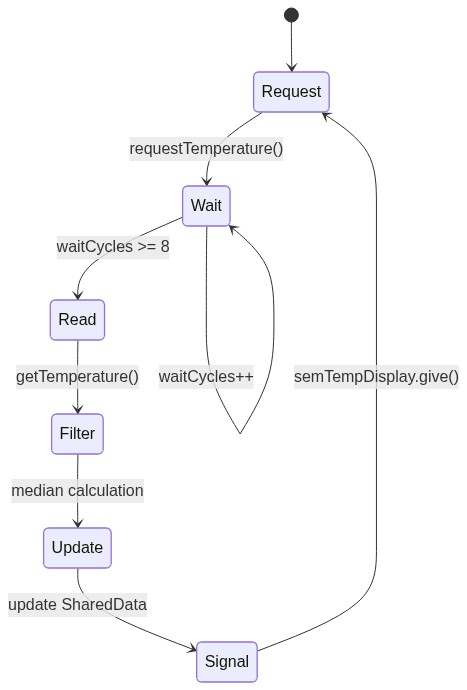
\includegraphics[width=0.4\textwidth]{24_state_temperature.png}
    \caption{State Machine - Temperature Sensor}
    \label{fig:state-temperature}
\end{figure}

This state machine shows the DS18B20 sensor states from initialization through temperature conversion and reading. It illustrates the non-blocking nature of the temperature acquisition process.

\begin{figure}[H]
    \centering
    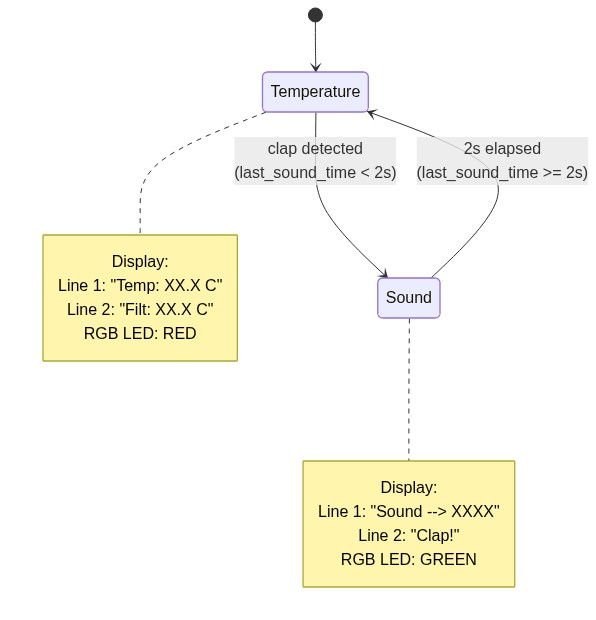
\includegraphics[width=0.4\textwidth]{25_state_display.png}
    \caption{State Machine - Display Mode}
    \label{fig:state-display}
\end{figure}

The diagram illustrates display mode transitions between temperature monitoring and sound event visualization. It shows how the display automatically switches based on recent system events.

\begin{figure}[H]
    \centering
    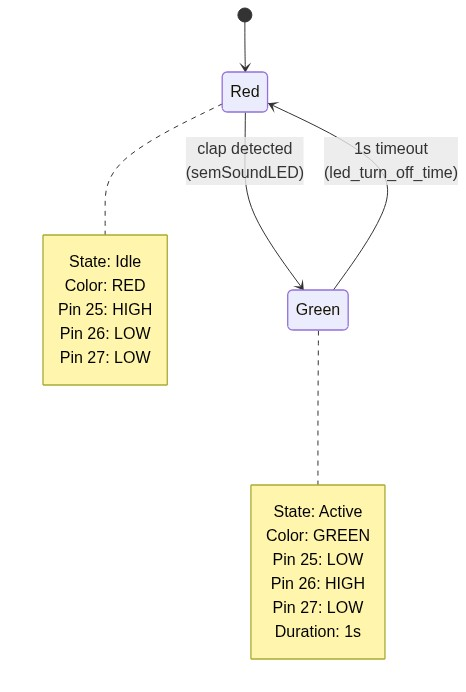
\includegraphics[width=0.4\textwidth]{26_state_rgb_led.png}
    \caption{State Machine - RGB LED}
    \label{fig:state-led}
\end{figure}

This state machine shows RGB LED transitions between red idle mode and green detection mode. It demonstrates the visual feedback system for monitoring system status.

\subsection*{5.7. Median Filter Implementation}

The median filter implemented for temperature readings uses a circular buffer of 5 samples. When a new temperature reading arrives, it is stored in the buffer and the oldest sample is discarded. The buffer is sorted, and the middle value (index 2) is selected as the filtered output. This approach effectively removes random outliers and noise while preserving the actual temperature trend without introducing significant phase delay.

\subsection*{5.8. System Timeline}

The system implements precise timing with four FreeRTOS tasks: vTaskDetect (20ms, priority 3) for sound acquisition, vTaskTemperature (100ms, priority 3) for temperature reading, vTaskDisplay (100ms, priority 2) for display updates, and vTaskRGBLED (continuous, priority 1) for LED control. All high-priority tasks use vTaskDelayUntil() for precise periodic execution, ensuring real-time responsiveness with input latency under 100ms.

% ============================================================================
% CHAPTER 6: ELECTRICAL DESIGN
% ============================================================================
\section*{6. Electrical Design and Hardware Implementation}

\subsection*{6.1. System Architecture Diagram}

\begin{figure}[H]
    \centering
    
\includegraphics[width=0.9\textwidth]{01_architecture.png}
    \caption{System Architecture - Dual Sensor Monitoring}
    \label{fig:architecture}
\end{figure}

This architecture diagram shows the complete system with hardware components, FreeRTOS tasks, and data flow paths. It illustrates the interaction between all system components.

\subsection*{6.2. Hardware Setup}

\begin{figure}[H]
    \centering
    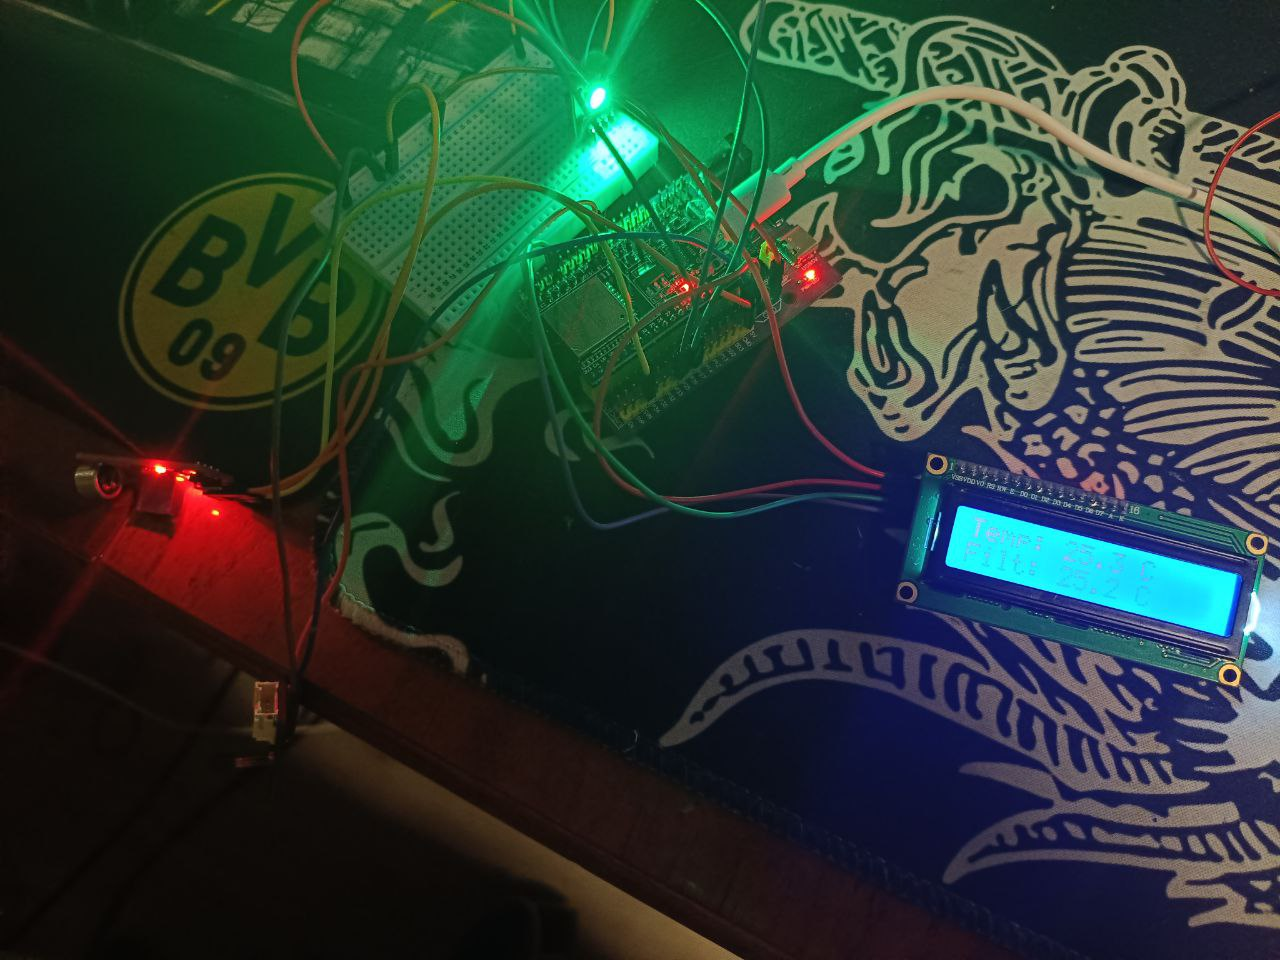
\includegraphics[width=0.45\textwidth]{../lib/lab3.2/tempreture-output-in-life.jpg}
    \caption{Hardware Implementation - Temperature Display Mode}
    \label{fig:hardware-temp}
\end{figure}

The photograph shows the complete system displaying temperature readings on LCD with RGB LED in red idle state. All components are properly connected and operational on the breadboard.

\begin{figure}[H]
    \centering
    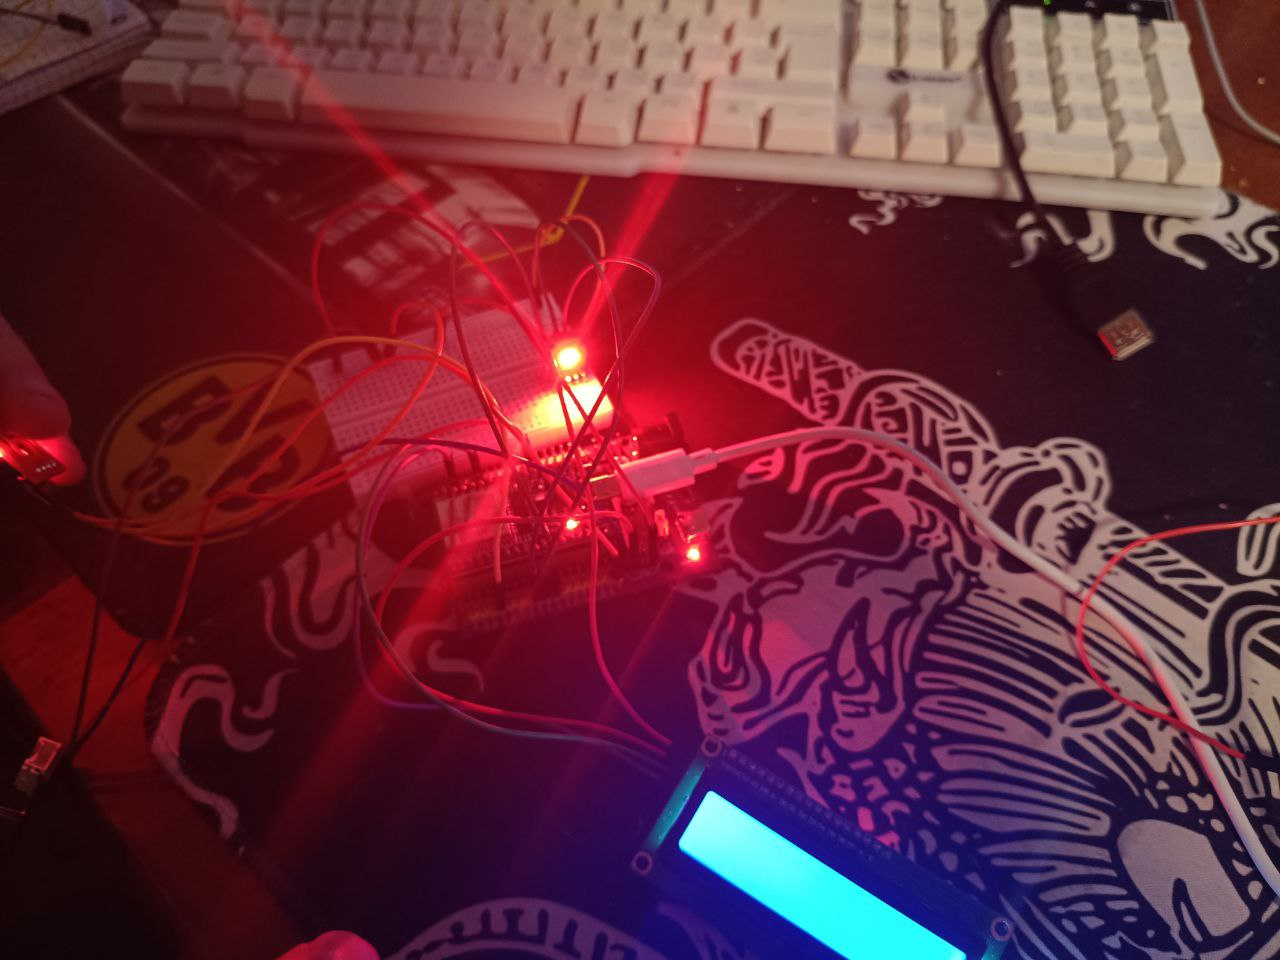
\includegraphics[width=0.45\textwidth]{../lib/lab3.2/sound-output-in-life.jpg}
    \caption{Hardware Implementation - Sound Detection Mode}
    \label{fig:hardware-sound}
\end{figure}

The photograph demonstrates the system during sound detection event with RGB LED in green state. The LCD shows the sound level value, and the RGB LED provides visual feedback.

\subsection*{6.3. DS18B20 Temperature Sensor Circuit}

The DS18B20 digital temperature sensor uses the OneWire protocol, requiring only three connections: VCC (3.3V or 5V), GND, and DATA (GPIO 4). A 4.7k$\Omega$ pull-up resistor must be connected between VCC and the DATA line for proper communication. The sensor provides temperature measurements with 9-12 bit configurable resolution (0.5°C to 0.0625°C precision) and operates in the temperature range of -55°C to +125°C. The OneWire protocol allows multiple sensors to be connected on the same bus, though this implementation uses a single sensor.

\subsection*{6.4. Sound Sensor Circuit}

The sound sensor module provides both digital (D0) and analog (A0) outputs. The digital output is connected to GPIO 12 and provides a threshold-based detection, while the analog output is connected to GPIO 34 (ADC1_CH6) and provides continuous voltage proportional to sound intensity. The analog output is read by the ESP32's 12-bit ADC, providing values from 0 to 4095 representing sound levels. The module includes a built-in potentiometer for adjusting the digital threshold sensitivity.

\subsection*{6.5. RGB LED Circuit}

The RGB LED uses three GPIO pins for individual color control: GPIO 25 (Red), GPIO 26 (Green), and GPIO 27 (Blue). Each LED color requires a current-limiting resistor (typically 220$\Omega$ to 330$\Omega$) to prevent excessive current. The common cathode configuration shares the ground connection, allowing individual color control through PWM. In this implementation, the RGB LED provides visual feedback: red for idle state and green for sound detection events.

\subsection*{6.6. LCD I2C Circuit}

The LCD 16×2 display is connected via I2C interface using GPIO 21 (SDA) and GPIO 22 (SCL). The I2C adapter board includes a PCF8574 I/O expander and typically includes 4.7k$\Omega$ pull-up resistors on SDA and SCL lines. The LCD operates at 5V but can communicate with the 3.3V ESP32 due to I2C's voltage compatibility. The display address is 0x27 (common for PCF8574 adapters).

% ============================================================================
% CHAPTER 7: IMPLEMENTATION AND TESTING
% ============================================================================
\section*{7. Implementation and Testing Results}

\subsection*{7.1. Temperature Monitoring Mode}

During normal operation (no sound events), the system displays temperature information as shown in Figure 15. The LCD shows both raw and filtered temperature values, demonstrating the effectiveness of the median filter in reducing measurement noise. Temperature readings are stable around 25.2°C with minimal variation, and the RGB LED maintains red color indicating idle state.

\subsection*{7.2. Sound Detection Mode}

When sound events are detected (analog value exceeds threshold of 1500), the system immediately switches display mode as shown in Figure 16. The LCD shows the sound level value "Sound --> XXXX" where XXXX represents the analog reading, the RGB LED changes to green color indicating sound detection, and the display maintains sound information for 2 seconds before returning to temperature monitoring.

\subsection*{7.3. Terminal Output Analysis}

\begin{figure}[H]
    \centering
    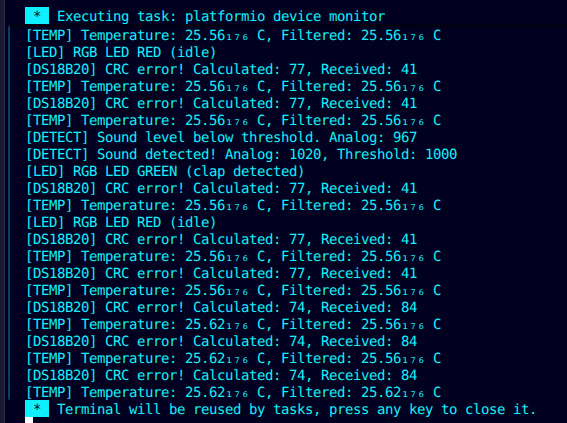
\includegraphics[width=0.9\textwidth]{../lib/lab3.2/Terminal-output.jpg}
    \caption{Terminal Output - System Operation}
    \label{fig:terminal-output}
\end{figure}

This terminal screenshot shows real-time system operation with temperature readings, sound detection events, and LED state changes. It demonstrates the system's ability to handle both sensor types simultaneously.

The terminal output demonstrates system behavior during operation. Temperature readings are shown as "[TEMP] Temperature: XX.XX°C, Filtered: XX.XX°C" with filtered values matching raw readings when stable. Sound detection events are logged as "[DETECT] Sound detected! Analog: XXXX, Threshold: 1500" with RGB LED changing from red to green. The system successfully handles both sensor types simultaneously with no blocking operations.

\subsection*{7.4. Test Results Summary}

The dual sensor monitoring system successfully achieves all specified requirements. Sound detection reliably triggers at threshold 1500 with 2000ms minimum interval between detections, temperature readings are stable with effective median filtering, display switching responds immediately to sound events and returns to temperature after 2 seconds, RGB LED provides clear visual feedback (red/green), and all four FreeRTOS tasks execute without blocking, maintaining system responsiveness. Input latency is under 100ms for both sensors, and memory usage remains efficient with approximately 30KB RAM consumption.

\subsection*{7.5. Known Issues and Limitations}

During testing, occasional CRC errors were observed in DS18B20 communication (calculated vs received CRC mismatch). These errors were addressed by implementing fallback temperature calculation and range validation, allowing the system to continue operation even with occasional communication errors. The median filter buffer is initialized with 20°C values, which may cause brief inaccuracy during system startup until the buffer is populated with actual measurements.

% ============================================================================
% CHAPTER 8: CONCLUSION
% ============================================================================
\section*{8. Conclusion}

This laboratory work successfully demonstrates the implementation of a dual sensor monitoring system using FreeRTOS on the ESP32 platform. The system effectively combines analog and digital sensor acquisition, non-blocking I/O operations, signal filtering with median filter, intelligent display management, and multi-state visual feedback. The modular architecture with clear separation between hardware abstraction and application logic allows for easy maintenance and extension. The use of FreeRTOS provides deterministic task scheduling and efficient resource management, enabling real-time responsiveness for both sensor types simultaneously.

Key achievements include successful implementation of non-blocking DS18B20 temperature acquisition without system blocking, effective median filtering reducing temperature measurement noise, intelligent display management that prioritizes time-critical sound events while maintaining regular temperature monitoring, reliable sound detection with configurable threshold and minimum interval, and stable multi-task operation with proper synchronization primitives.

The system demonstrates practical applications in environmental monitoring, security systems, and IoT devices where multiple sensor types must be monitored simultaneously with real-time response capabilities. Future enhancements could include additional sensors, data logging to external storage, wireless transmission of sensor data, and adaptive thresholds based on ambient conditions.

% ============================================================================
% CHAPTER 9: AI ASSISTANCE
% ============================================================================
\section*{9. AI Assistance}

This laboratory report was generated with assistance from artificial intelligence tools. The AI system helped in several aspects of document creation:

\subsection*{9.1. Text Generation}

The AI assistant contributed to generating the textual content of the report, including the introduction, analysis of domain situation, resource descriptions, and conclusion sections. The text was structured according to academic standards for technical documentation, ensuring proper formatting and organization of information.

\subsection*{9.2. Structure and Organization}

The report structure was designed to follow the template established in Laboratory Work 3.1, adapted for the dual sensor monitoring system. The AI system assisted in organizing content into logical sections, including introduction, domain analysis, resources, task description, architectural design, electrical design, implementation and testing, and conclusion. Each section was structured to provide clear, concise information appropriate for technical documentation.

\subsection*{9.3. Diagram Descriptions}

The AI system provided descriptive text for all figures, diagrams, and photographs included in the report. These descriptions (1-3 sentences each) explain the purpose and content of each visual element, enhancing document readability and comprehension. The descriptions were written in plain text format below each figure to maintain document flow and readability.

\subsection*{9.4. Technical Content}

Technical information about the system architecture, FreeRTOS implementation, sensor protocols, and electrical circuits was synthesized from the actual code implementation and hardware setup. The AI assistant helped organize this information into a coherent narrative that demonstrates understanding of the underlying technologies and design decisions.

\subsection*{9.5. Documentation Standards}

The report follows standard technical documentation practices, including proper LaTeX formatting, figure referencing, table organization, and citation of diagrams. The AI system ensured consistency in terminology, formatting, and presentation style throughout the document.

\end{document}
